\chapter{CouchDB-Umfeld}
\label{Umfeld}

\section{Security}

\subsection{Absicherung des CouchDB-Servers}

\subsection{Absicherung der Administrationsoberfläche}

Als moderne Management-Oberfläche für CouchDB steht die Web-Anwendung \emph{Fauxton} zur Verfügung. Diese kann einfach als npm-Paket installiert werden und ist danach über HTTP erreichbar \cite{fauxton:overview}. Welcher Webserver die Anwendung in diesem Fall ausliefert, ist nicht klar. Um nicht durch dessen eventuelle Sicherheitslücken gefährdet zu werden, muss zwischen diesen Webserver und das Internet ein sogenannter \emph{Reverse Proxy} geschaltet werden.

\begin{figure}[htb]
	\centering
	\caption{Netzwerkdiagramm für den Einsatz eines Reverse Proxy}
	\label{fig:reverseproxy}
	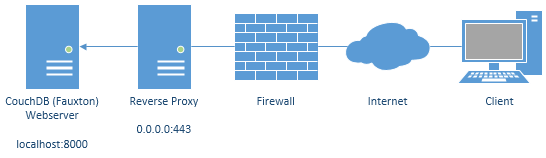
\includegraphics[width=\textwidth]{\figdir/Reverse_Proxy.png}
\end{figure}

Abbildung \ref{fig:reverseproxy} zeigt in einem Netzwerkdiagramm, wie der CouchDB-Server in diesem Projekt mit dem Internet verbunden ist. Eine Firewall lässt von außen nur Zugriffe über Port 443 (HTTPS) zu. Der Reverse Proxy lauscht an diesem Port und reicht alle Anfragen an den CouchDB/Fauxton-Webserver an Port 8000 weiter. Dabei wird gleichzeitig die TLS-Verbindung terminiert. Somit muss Fauxton keine TLS-Verbindungen aufbauen und braucht keine sicherheitskritischen Informationen über die verwendeten Zertifikate.

% Todo: Quellen, Passwörter etc.